\documentclass{beamer}
 
\usepackage[utf8]{inputenc}
\usepackage{verbatim}
\usepackage{listings}
\usetheme{Madrid}
 
%Information to be included in the title page:
\title{W05 Sep 16 (D1) Matching sequences detector}
\author{Biplav Karna}
\institute{USN Kongsberg}
\date{2019}
 
 
 
\begin{document}
 
\frame{\titlepage}
 
\begin{frame}
\frametitle{Overview}
\tableofcontents
\end{frame}

\section{Problem Description}
\begin{frame}
\frametitle{Matching Sequence Detector}
\includegraphics[width=\textwidth, height=0.8\textheight] {../diagrams/D1-sep16-prob.png}
\end{frame}
 
\section{State Diagram}
\begin{frame}
\frametitle{State Diagram}
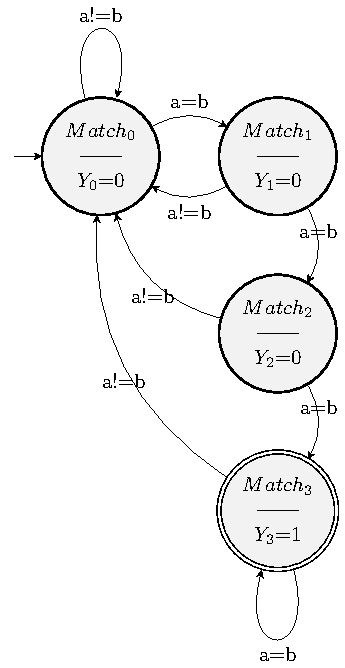
\includegraphics[height=0.8\textheight] {../diagrams/state-diagram.pdf}
\end{frame}
 
\section{Asm Diagram}
\begin{frame}
\frametitle{Asm Diagram}
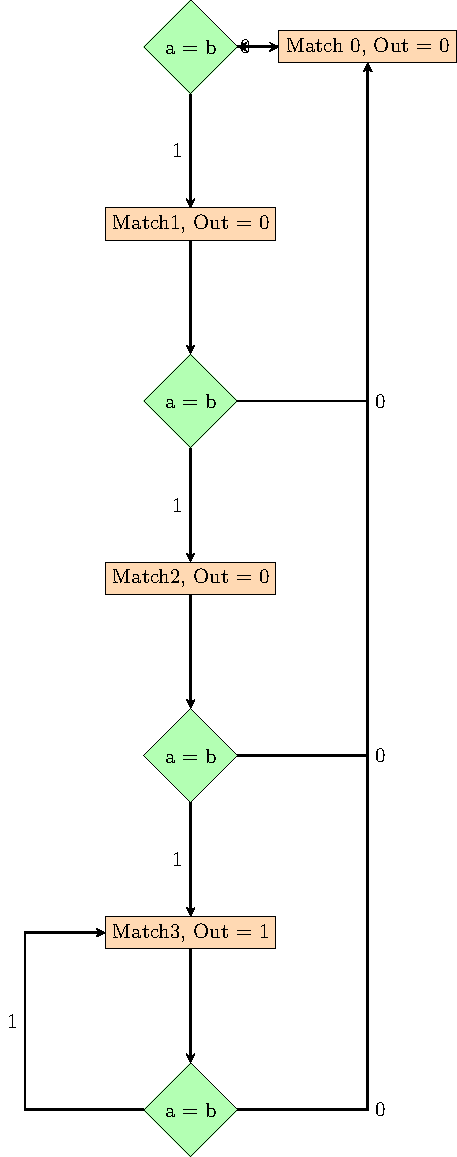
\includegraphics[height=0.8\textheight] {../diagrams/Asm-diagram.pdf}
\end{frame}

\section{Source Code}
\subsection{dff.vhd}
dff.vhd
\begin{tiny}
\lstinputlisting[language=Vhdl,breaklines=true]{../src/dff.vhd}
\end{tiny}

\break

\subsection{one-bit-comparator.vhd}
one-bit-comparator.vhd
\begin{tiny}
\lstinputlisting[language=Vhdl,breaklines=true]{../src/one-bit-comparator.vhd}
\end{tiny}
\break

\subsection{seq\_detect\_fsm.vhd}
\begin{small}
seq\_detect\_fsm.vhd
\end{small}
\begin{tiny}
\lstinputlisting[language=Vhdl,breaklines=true]{../src/seq_detect_fsm.vhd}
%\verbatiminputv{../src/seq_detect_fsm.vhd}
\end{tiny}


\break
\section{Simulation}
\subsection{Source Code}
\begin{small}
Source ( seq\_dectect\_fsm\_tb.vhd )
\end{small}
\begin{tiny}
\lstinputlisting[language=Vhdl,breaklines=true]{../testbench/seq_dectect_fsm_tb.vhd}
%\verbatiminputv{../src/seq_detect_fsm.vhd}
\end{tiny}

\break

\subsection{Output}
\begin{frame}
\frametitle{Output}
\includegraphics[width=\textwidth,height=0.8\textheight] {../diagrams/simulation.png}
\end{frame}

\section{Thanks}
\begin{frame}
\frametitle{Thanks}
\includegraphics[width=0.4\textwidth,height=0.6\textheight]{/Users/biplavkarna/Pictures/namaste.png}
\end{frame}

\end{document}
